\section{Implementation}

The project implementation is split into two primary sections. The first is the
scoring only implementation, the second is the parsing and scoring
implementation. The scoring only implementation comprised the entire initial
project plan and involved porting the existing scoring code from C++ to OpenCL.
After the implementation of the scoring code, and the initial analysis of
results was conducted, it was determined that the parsing code (also written in
C++) was the bottleneck to the system and the project then began to investigate
also porting the parsing code to OpenCL.

A note on terminology: When a contiguous block of memory is allocated on the
host device it is normally referred to as an array. When the array is
transferred to an OpenCL device it is referred to as a buffer. These are
functionally the same with the primary distinction being where they are
allocated.

\subsection{All implementations}

Most OpenCL applications are implemented in much the same way from the host
code's perspective. There is a significant amount of boiler plate code to detect
OpenCL platforms and devices available on the target system. Each device that is
going to be used needs it's own command queue. An OpenCL command queue is as the
same suggests, any data transfers or kernel executions are placed on the
device's command queue and executed in order of arrival to the queue (although
out of order execution is possible). Command queues, memory, program, and kernel
objects are all managed by an OpenCL context. The kernel itself also has to be
compiled, it is read in from disk as a string and built for the required
devices. This is what allows a single kernel to run on any available device
selected, it's compiled at run time. After compilation is completed, the
kernel's arguments are set to the appropriate device buffers. The host's arrays
that contain data the kernel needs are then transferred to the device's buffers
and the kernel is executed. After the kernel has finished executing, any buffers
relating to results, in this case the document scores, are written back by en-
queuing a read buffer command.

As discussed in the background, the Naive-Bayes classifier makes use of a
profile. This is a 128MB file containing the terms and associated term weights.
This is read in from disk by the C++ host device code, and passed in as a buffer
of unsigned long values to the OpenCL kernel. It does not change between
invocations of the kernel, as all sets of documents are scored using the same
profile.

The use of a bloom filter was also discussed in the background. This is a 4KB
array of bit values used by the OpenCL kernel to see if there is a chance that
the document term being scored exists in the profile. As with the profile, this
is read in from disk and passed in as a buffer to the OpenCL kernel. It also
does not change between invocations of the kernel because the profile does not
change.

OpenCL host code is summarised in the pseudo-code in
Figure~\ref{fig:openCLPseudocode}.

\begin{figure}
\begin{verbatim}
// One time set up
platforms = getPlatforms()
devices = getDevices(platforms[0])
context = createContext(devices)
queue = createCommandQueue(context, devices[0])
program = buildProgram(context, sourceCode)
kernel = createKernel(program, kernelMethodName)

// repeat for each buffer
buffer1 = createBuffer(context, options, size)
setArg(kernel, 1, buffer1)
writeBuffer(buffer1)

resultsBuffer = createBuffer(context, options, size)
setArg(kernel, n, resultsBuffer)

// Execute kernel and get results back
enqueueKernel(queue, kernel)
readBuffer(resultsBuffer)
\end{verbatim}
\caption{OpenCL Host Pseudo-code}
\label{fig:openCLPseudocode}
\end{figure}

\subsection{Scoring Only}

In addition to the profile and bloom filter, the scoring only implementation
reads in the parsed document terms from disk. These are passed to the OpenCL
kernel and are used to calculate a document's score.

The array of terms is a one dimensional array thus the C++ code has to iterate
over the array and find the beginnings of documents to know how many work items
to create (one per document) and over what range of terms represent each
document. This simply involves the creation of indexes containing the location
of terms with length 0 as this was used to delimit document beginnings. The
array of document marker addresses is prefixed by the number of documents and
has the total number of terms added to the end of the array. The total term
number is required by the work item scoring the last document as there is no
next document to determine where to stop scoring terms at. This buffer is also
transferred to the device.

All buffers are read only with the exception of the scores buffer. This is a
write-only buffer with length equal to the number of documents being scored. It
is this buffer that the kernel writes the results to and is the only buffer that
needs to be written back to the host memory after kernel execution.

After the kernel has the arguments set to the appropriate buffer, and the data
has been transferred to the device the kernel can execute. During kernel
execution, each work item iterates of the terms for their associated document. A
work item knows which document to score because the location of the document
starting term is the work item's ID + 1, up to the work item's ID + 2. Each term
in this range is scored and the total score for the document is stored in a
scores buffer at location equal to the work item's ID.

The OpenCL kernel code is summarised in the pseudo-code in
Figure~\ref{fig:scoringPseudocode}.

\begin{figure}
\begin{verbatim}
documentNumber = get_global_id(0) + 1 // work item ID
startIndex = docAddresses[documentNumber]
endIndex = docAddresses[documentNumber + 1]
score = 0
for (term in terms[startIndex..endIndex]) {
    generateNGrams(term)
    for (ngram in ngrams) {
        address = getTermAddress(ngram)
        profileEntryVector = profile[address]
        for (i = 0; i < 4; i++) {
            profileEntry = profileEntryVector[i]
            if (profileEntry contains ngram) {
                score += getWeight(profileEntry)
            }
        }
    }
}
scores[documentNumber -1] = score
\end{verbatim}
\caption{Scoring Pseudo-code}
\label{fig:scoringPseudocode}
\end{figure}

After the kernel has finished executing, and the scores buffer has been written
to a host device array, the actual classifications of each document is
recovered. A document is classed as significant (spam in the spam or not spam
example) if the score is above a certain threshold.

\subsection{Parsing and Scoring}

For the parsing and scoring version, the host code is very similar. The only
differences relate to the documents themselves. For scoring only, the documents
were already parsed and represented by terms. For parsing and scoring, the plain
text is instead read in. The TREC data collection is read in as a single text
file and passed to the OpenCL kernel as-is. For the document marker array,
instead of detecting zero length terms, the C++ code searches through the plain
text and stores the character locations where the sub-string ``$<$DOC$>$''
begins. This sub-string acts as a direct replacement to the zero length term
locations, and is transferred to the OpenCL kernel in the same way.

Again, each work item is responsible for a single document. During the kernel
invocation, each work items parses the documents character by character and, as
soon as a full term has been parsed, scores the term. A term is ready to score
when a white space character has been reached, and the term is of non-zero
length. Any characters inside tags, for instance the start and end doc tags, are
ignored. After all characters have been parsed, the scores are stored in the
same way as the scoring code.

After the kernel has finished, the scores are written back to the host and the
classifications are calculated as before.

The OpenCL kernel code is summarised in the pseudo-code in
Figure~\ref{fig:parsingScoringPseudocode} where to5BitEncoding(char) is the
Baudot encoding discussed and shown in Figure~\ref{baudotCode}, scoreTerm(term)
contains the profile lookup and scoring addition code from
Figure~\ref{fig:scoringPseudocode}, and updateState(state) works out the parser
state machine transition based on the current state, and what character has just
been found. States tell the parser to either skip characters, write characters
to the term, `flush' the term (aka score the term), or that a tag has been
encountered.

\begin{figure}
\begin{verbatim}
documentNumber = get_global_id(0) + 1 // work item ID
startIndex = docAddresses[documentNumber]
endIndex = docAddresses[documentNumber + 1]
state = SKIPPING
score = 0
for (char in documents[startIndex..endIndex]) {
    if (char is alphanumeric) {
        updateState(state, 0)
        if (state is WRITING) {
            term += to5BitEncoding(char)
        }
    } else if (char is whitespace) {
        updateState(state, 2)
        if (length(term) > 0 and state is FLUSHING) {
            score += scoreTerm(term)
            term = 0 // Parse a new term now
        }
    } else if (char is '<') {
        updateState(state, 3)
    } else if (char is '>') {
        updateState(state, 4)
    } else {
        updateState(state, 1)
    }
}
\end{verbatim}
\caption{Parsing and Scoring Pseudo-code}
\label{fig:parsingScoringPseudocode}
\end{figure}

\section{Optimisations}

OpenCL kernels can run on any device with a suitable compiler. This portability
is helpful when using different types of devices which may come from a multitude
of vendors. This portability has a cost however, there is no guarantee that the
kernel will run well. For instance, CPUs and GPUs are significantly different in
terms of how they cache and GPUs are more favourable for smaller tasks which can
be done in parallel. This requires a developer to consider the architectural
differences of different devices and tune each kernel for each device. Two
significant optimisations that were employed during this project are discussed
below. The ``Local Size'' optimisation involves changing the number of work
items in a work group to suit the target device. The second optimisation,
``Mapped Buffers'', is a simple optimisation to remove any unnecessary data
transfers.

A third optimisation, using bloom filters, was also employed however this is
discussed in the next section as the three bloom filters, and their effect on
performance demands a more thorough analysis.

\subsection{Local Size}

When executing a kernel, the host code specifies the number of work items to
create (the global size) and the number of work items per work group (the local
size). With a single work group being assigned to a single compute unit, and one
compute unit being able to have multiple work groups simultaneously, the local
size can have a significant effect on kernel performance. Different devices
react better to larger work groups, for instance GPUs which can use large work
groups to improve latency hiding. The type of algorithm also has an affect on
the optimal local size, certain characteristics prefer larger work groups to
others. For these two reasons, there is no hard and fast rule dictating what
local size to use for what device and algorithm, experimentation to fine tune
the kernel is the only way.

Local size can have a value from 1 up to 512, 1024, or 2048, depending on the
device. This is specified by the ``CL\_DEVICE\_MAX\_WORK\_GROUP\_SIZE'' constant
that can be queried at runtime. The value is typically a power of two. The only
other restriction to the local size is that it must be a factor of the global
size (for instance a local size of 64 and a global size of 4096). Given that
global size can be any number, for instance the number of documents, it is
common to round up the global size to the nearest number that makes local size a
factor. The kernel can then conduct a bounds check and have the few work items
extra to return straight away. These extra work items do not affect performance
as they only appear as part of the last work group.

Another benefit of modifying the local size is occupancy of a compute unit. A
work item uses a certain amount of memory, its private variables. A compute unit
only has a limited capacity for these variables thus, based on the kernel code,
can only simultaneously handle a maximum number of work items. Say the compute
unit can handle 2048 work items at one time, thus any combination of local size
(assuming powers of two) will allow for 100\% occupancy of the compute unit (say
two work groups with size 1024 work items). If the unfortunate situation occurs
where 2040 work items can be handled, a local size of 1024 will result in a
single work group being handled by the compute unit resulting in just over 50\%
occupancy. If the local size was 32, there would be 63 work groups assigned to
the compute unit, resulting in just under 99\% occupancy. A higher occupancy can
make better use of a computes resources and increase overall throughput.

Specific to this project, the Tesla C2075 and Intel Xeon Phi 5110P performance
for the parsing and scoring kernel had an in-depth analysis regarding to their
local size. It was found that the Tesla C2075 reacted well to a large local
size, likely to assist with latency hiding of memory accesses, and achieved the
best performance with a local size of 128.

Graph of local size effect on the Tesla C2075 is shown in
Figure~\ref{fig:teslaLocalSize}. There is a gradual improvement in performance
up to a local size of 128 where performance then starts to drop off for larger
work groups. In this example, choosing a poor work group size (1) will increase
the time to score a set of documents by a factor of five.

\begin{figure}[H]
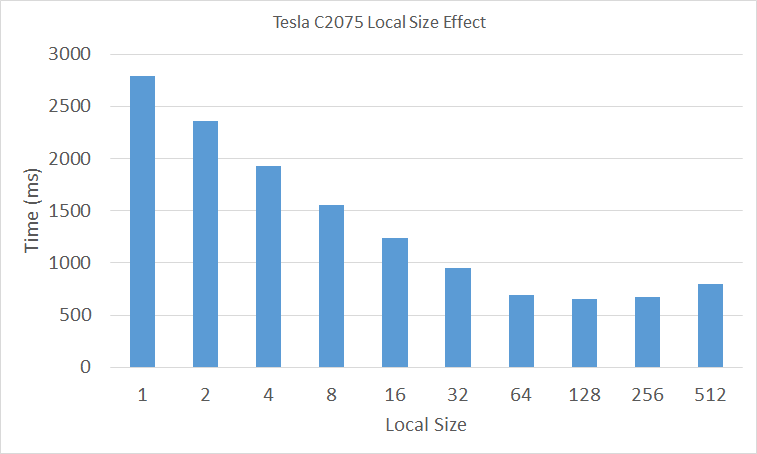
\includegraphics[width=\linewidth]{images/teslaLocalSize.png}
\caption{Tesla C2075 Local Size Effect}
\label{fig:teslaLocalSize}
\end{figure}

The Intel Xeon Phi 5110P reacted best to small local sizes, with a big jump in
performance when going from a local size of 16 to 8. The optimum performance was
with a local size of 4, which is likely due to the 4-way hyper-threading
employed by the device.

Graph of local size effect on Intel Xeon Phi is shown in
Figure~\ref{fig:phiLocalSize}. There is a gradual improvement in performance as
the local size is reduced from 512 to 16. Interestingly, there is a massive
improvement when moving to a local size of 8, the performance increases by over
a factor of two. In this example, choosing a poor work group size (512) will
increase the time to sore a set of documents by a factor of three.

Regarding overall performance changes, the Tesla C2075 has a greater benefit of
an optimum local size to the Intel Xeon Phi however the Intel Xeon Phi has a
much sharper reaction when nearing the optimal value whereas the Tesla has a
more gradual change.

\begin{figure}[H]
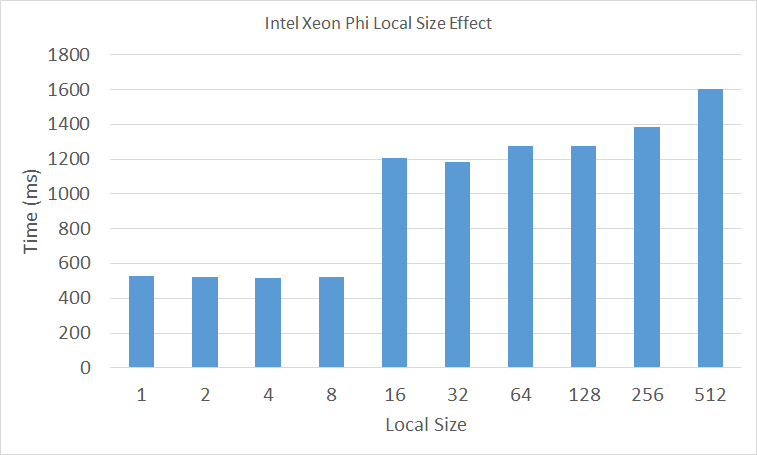
\includegraphics[width=\linewidth]{images/phiLocalSize.png}
\caption{Intel Xeon Phi 5110P Local Size Effect}
\label{fig:phiLocalSize}
\end{figure}

\subsection{Mapped Buffers}

When using an accelerator device such as a graphics card, the data used by the
kernel has to be transferred over the PCI-E bus by en-queueing a write buffer
command. This incurs an unavoidable time cost as the PCI-E bus has limited
bandwidth. When running OpenCL code on the CPU this is not the case as the
OpenCL buffers can stay in primary memory. Unfortunately, the write buffer
command does not realise that this is the case, and when executing a write
buffer command for the CPU, copies the host array from primary memory to another
location in primary memory. As well as duplicating memory usage this incurs an
avoidable time cost.

The solution to the issue is to map the OpenCL buffer to the host array. This is
done by executing an en-queue map buffer command. The OpenCL buffer can then
read from the host address space and removes the requirement for the unnecessary
duplication of memory. The benefits of mapping a buffer is essentially a free
lunch as the call takes an insignificant amount of time to execute.
